\documentclass{scrartcl}

\usepackage{helvet}
\usepackage[T1]{fontenc}
\usepackage[ngerman]{babel}
\usepackage[utf8]{inputenc}
\usepackage{enumitem}
\usepackage{hyperref}
\usepackage{graphicx}
\renewcommand{\familydefault}{\sfdefault}
%----------------------------------
% thomi fa list implementation
%----------------------------------

\newlist{falist}{enumerate}{2}
\setlist[falist,1]{label={/FA\arabic{falisti}\arabic{falistii}/},align=left,labelwidth=17pt,labelsep=3pt,leftmargin=20pt}
\setlist[falist,2]{label={/FA\arabic{falisti}\arabic{falistii}/}}%,align=left,labelwidth=17pt,labelsep=3pt,leftmargin=0pt}

\usepackage{chngcntr}
\counterwithin{falistii}{falisti}

\newlist{pdlist}{enumerate}{2}
\setlist[pdlist,1]{label={/PD\arabic{pdlisti}\arabic{pdlistii}/},align=left,labelwidth=17pt,labelsep=3pt,leftmargin=20pt}
\setlist[pdlist,2]{label={/PD\arabic{pdlisti}\arabic{pdlistii}/}}%,align=left,labelwidth=17pt,labelsep=3pt,leftmargin=0pt}
\counterwithin{pdlistii}{pdlisti}

\newlist{nflist}{enumerate}{2}
\setlist[nflist,1]{label={/NF\arabic{nflisti}\arabic{nflistii}/},align=left,labelwidth=17pt,labelsep=3pt,leftmargin=20pt}
\setlist[nflist,2]{label={/NF\arabic{nflisti}\arabic{nflistii}/}}%,align=left,labelwidth=17pt,labelsep=3pt,leftmargin=0pt}
\counterwithin{nflistii}{nflisti}

\newlist{telist}{enumerate}{2}
\setlist[telist,1]{label={/T\arabic{telisti}\arabic{telistii}/},align=left,labelwidth=17pt,labelsep=3pt,leftmargin=20pt}
\setlist[telist,2]{label={/T\arabic{telisti}\arabic{telistii}/}}%,align=left,labelwidth=17pt,labelsep=3pt,leftmargin=0pt}
\counterwithin{telistii}{telisti}

\begin{document}

\begin{titlepage}

\title{Pflichtenheft: Lambda - Das Spiel, Team Dirty Bit Misses}
\author{Luca Becker, Henrike Hardt, Larissa Schmid, Adrian Schulte, Maik Wiesner}
\date{\today}

\maketitle
\thispagestyle{empty}

\end{titlepage}

\clearpage

\tableofcontents
\thispagestyle{empty}

\clearpage
\setcounter{page}{1}






% ---------------
% Einleitung
% ---------------

\section{Einleitung}

Der derzeitige und auch kommende Ingenieursmangel in Deutschland ist
schon seit Langem Thema in den Medien. „Auf jeden Bewerber kommen
etwa 4 freie Stellen“%
\footnote{http://www.ingenieurwesen-studieeren.de/ingenieurmangel/%
}, „jeder zweite angehende Ingenieur bricht sein Studium ab“%
\footnote{http://www.zeit.de/studium/hochschule/2013-10/ingenieure-unis-fachkraeftemangel%
}, all diese Nachrichten geben Grund zur Sorge in Hinblick auf Deutschland
als Technologiestandort. Unsere Volkswirtschaft beruht nicht mehr
auf Wertschöpfung aus dem ersten und zweiten, sondern vor allem aus
dem dritten Sektor – damit dies weiterhin funktionieren kann, werden
vor allem Ingenieure benötigt. Doch an dem derzeitigen Mangel ist
nicht nur die Überalterung unserer Gesellschaft schuld, sondern vor
allem auch die fehlende Begeisterung von Jugendlichen für die sogenannten
MINT-Fächer (Mathematik, Informatik, Naturwissenschaft, Technik).
Um Deutschland als Standort auch weiterhin wettbewerbsfähig zu halten,
ist es somit wichtig, Kinder schon frühestmöglich spielerisch an Fragestellungen
aus diesen Bereichen heranzuführen. 

In der Informatik ist der Lambda-Kalkül ein wichtiges Konstrukt, der
zum Beispiel die Entwicklung funktionaler Programmiersprachen wesentlich
beeinflusst hat. Obwohl er damit eine große Bedeutung hat und sehr
mächtig ist in Bezug auf sowohl die Theoretische Informatik als auch
funktionale Programmierung, so sind die grundlegenden Regeln dennoch
nicht allzu komplex und leicht verständlich. 

Um Kindern also schon im Grundschulalter eine erste Auseinandersetzung
mit Themen der Informatik und damit auch der Ingenieurswissenschaften
zu bieten, eignet sich der Kalkül also sehr gut. Unsere nachfolgend
dargelegte Visualisierung der Funktionsweise des Kalküls mithilfe
von einfachen Formen und sie ineinander umwandelnden Maschinen ist
dabei besonders kindgerecht, wodurch der Kalkül anhand von einfachen
Lambda-Ausdrücken einfacher verstanden und verinnerlicht werden kann.
Diese Idee soll nun als Android-App umgesetzt werden, sodass Kinder
selbständig spielen können, der Fortschritt im Spiel aber auch jederzeit
durch Eltern oder Lehrkräfte einsehbar ist. 

\clearpage








% ---------------
% Zielbestimmungen
% ---------------

\section{Zielbestimmungen}


Die Kinder sollen durch das Spiel in die Lage versetzt werden, sich die Prinzipien des Lambda Kalküls spielerisch zu erarbeiten ohne über Vorkenntnisse zu verfügen.

\subsection{Musskritieren}

\begin{enumerate}
	\item \label{muss:vermittelnlamba}Spielerisches Vermitteln des Lambda Kalküls für Kinder ab acht Jahren
	\item \label{muss:simulationandroid}Das Spiel muss in der Simulationsumgebung von Android laufen
	\item \label{muss:touchinterface}komplett über das simulierte Touchinterface bedienbar sein
	\item \label{muss:mvc}eine modulare Architektur besitzen (z.B. Model-View-Controller-Prinzip)
	\item \label{muss:5indilevel}mindestens fünf individuelle Level
	\item \label{muss:tutorial}Tutorial Level
\end{enumerate}

\subsection{Wunschkriterien}

\begin{enumerate}
	\item \label{wunsch:werkstatt}Werkstatt zum Umbauen von Maschinen
	\item \label{wunsch:highscore}Highscore-Tabelle
	\item \label{wunsch:challengemode}Challengemode mit Zeitdruck
	\item \label{wunsch:multilang}Auslieferung in mehreren Sprachen
	\item \label{wunsch:8bit}8-Bit Grafik
	\item \label{wunsch:multiplechar}Mehrere Spielcharaktere (männlich, weiblich)
	\item \label{wunsch:multiplemode}Mehrere Spielmodi (siehe Aufgabentyp \ref{aufgabentyp:fehlerfindung})
    \item \label{wunsch:story}Begleitende Story
    \item \label{wunsch:erweiterndeLevelelemente}Erweiternde Levelelement, z.B. Leitern, Aufzüge usw.
\end{enumerate}

\subsection{Abgrenzungskritieren}

\begin{enumerate}
	\item Kein Onlinemodus
	\item Kein Multiplayer Modus
	\item Keine vorgesehene Kompatiblität mit anderen Geräten/Betriebssystem ohne Emulation
\end{enumerate}

\clearpage










% ---------------
% Spielaufbau
% ---------------

\section{Spielaufbau}

\subsection{Spielprinzip}
Das Spielprinzip beruht auf dem Bewegen von Blöcken, indem der Spieler die Blöcke hochhebt und wieder absetzt. Der Spieler muss die verschiedenen Teile des Spieles, die Maschinen(), die Maschinen-Cluster() und die Metallstücke, in die dafür vorgesehenen Positionen bringen. Hat er alle Teile in die richtigen Positionen gebracht, öffnet sich die Tür zum nächsten Level.


\subsection{Spielelemente}

Zu Beginn eines Levels wird die Spielerfigur angezeigt und bewegt zweidimensional durch die Welt und wird vom Spieler gesteuert.

\begin{description}
	\item[Spielerfigur] bewegt sich durch die Welt, sammelt Gegenstände um mit diesen die Levelquest zu lösen
	\item[Leben] Jeder Spieler hat je Level drei Leben, die er verlieren kann, wenn er ins Wasser fällt
	\item[Spielwelt] zweidimensionale Spielwelt auf einem Raster basierend, in der sich der Spieler bewegt
	\item[Spielebenen] verschiedene Ebenen in der Spielwelt auf die der Spieler springen kann, sie sind auf einem Raster angeordnet
		\begin{enumerate}[label=\arabic*]
			\item Landebenen: Auf diesen Ebenen liegen die Collectable Items
			\item Wasserebenen: Fällt der Spieler in das Wasser, muss er wieder am linken unteren Rand anfangen und er verliert ein Leben, hat er kein Leben mehr, so muss er das Level neu beginnen
		\end{enumerate}
	\item[Collectable Items] \label{elemente:collectable}sind in der Spielwelt verteilt und müssen von der Spielfigur eingesammelt werden um im Rätselteil eingesetzt zu werden. Diese bestehen aus:
	\begin{enumerate}[label=\arabic*]
		\item Maschinen (entspricht der Abstraktion)
		\item Metallstücke (entspricht der Variablen)
		\item Maschinen-Cluster (entspricht der Applikation)
	\end{enumerate}
	\item[Levelquest] sind gegebene Aufgaben die zum Abschließen des Levels erfüllt werden müssen
	\item[Leveltür] bildet den Abschluss eines Levels. Sobald alle Quests in dem Level gelöst wurden wird die Tür freigeschaltet
\end{description}

\subsection{Regeln}

\begin{description}
	\item[Spielregeln] \label{spielaufbau:Spielregeln} Die Spielfigur beginnt an der unteren, linken Ecke der Spielwelt und muss es schaffen die Tür an der rechten unteren Ecke zu öffnen. Dies gelingt ihm in dem er die Teile des Spieles an die richtige Position bringt.\\
	Er muss neben einem Teil stehen, um es hochheben zu können.\\
	Der Spieler kann nur ein Teil gleichzeitig bewegen, sobald er etwas trägt, muss er dies erst wieder ablegen, um ein anderes Teil hochheben zu können. \\
	Um auf die oberen Ebenen der Spielwelt zu gelangen, kann die Spielfigur springen, dabei ist zu beachten, dass die Figur nur eine feste Höhe hochspringen kann und er somit auf zu Ebenen, außerhalb seiner Reichweite, nicht durch einfaches Springen gelangen kann. Die Figur kann auch springen wenn sie etwas in den Händen trägt (dabei kann es zu einer geringen Trägheit kommen, z.B. ungenauere Spielsteuerung).\\
	Sind alle Teile in die freien Felder positioniert, wird ausgewertet, ob die Maschinen und Metallstücke an den richtigen Positionen stehen und der $\lambda$-Kalkül erfüllt ist. Stehen die Elemente an der richtigen Position, geht die Tür zum nächsten Level auf.

	
	\item[Die Verarbeitungsregel der Maschinen] Die Verarbeitung der einzelnen Metallstücke erfolgt in fester Reihenfolge().\\
	Es wird immer nur ein Metallstück zu einem bestimmten Zeitpunkt verarbeitet.\\
	Wie das Objekt verarbeitet wird bestimmt die jeweilige Maschine.\\
	Die Maschinen werden in fester Reihenfolge () angeordnet und verarbeiten nacheinander die gegebenen Metallobjekte.\\
	Dabei kann jede Maschine nur ein Objekt verarbeiten, nachdem sie dieses Metallobjekt verarbeitet hat verschwindet sie.\\
	Jede Maschine kann Form, Farbe/Muster und Anzahl des zu verarbeitenden Objekts verändern. Hierbei ist zu beachten das eine Maschine auch ein Objekt komplett entfernen kann. Was eine Maschine genau am zu verarbeitenden Objekt verändert ist durch ihr aussehen eindeutig bestimmt.\\
	Das verarbeitete Objekt landet im Output-Bereich unterhalb des Maschinen-Bereichs, dieser ist gleichzeitig Input-Bereich des nachfolgenden Maschinenbereichs.\\
	Sind keine Maschinen mehr im Maschinen-Bereich vorhanden, so werden alle noch im Input-Bereich liegenden Metallobjekte ohne Verarbeitung in den darunter liegenden Output-Bereich verschoben. Anschließend beginnt der nächste darunterliegende Maschinen-Bereich nach selben Regeln seine Arbeit.\\
	Sollte unterhalb des aktuellen I/O Bereichs kein Maschinen-Bereich mehr vorhanden sein, so ist das Level Beendet und der aktuelle Output wird mit den Zielvorgaben vom Level beginn verglichen.
	
	\item[Sonderfälle/regeln:] Sollten in einem Maschinen-Bereich noch Maschinen vorhanden sein, im zugehörigen Input-Bereich jedoch keine Metallobjekte mehr, so verschwindet entsprechende Maschine einfach.\\
	Sollte die im Maschinen-Bereich aktuell arbeitende Maschine ein Ampel-Konstrukt sein, so wird vor Verarbeitung des aktuellen Objekts im Input-Bereich der im Ampel-Konstrukt dargestellte Maschinen-Cluster minimiert, sodass er durch eine Maschine dargestellt wird. Dann wird das Aktuelle Metallobjekt von der Minimalen Maschine im Ampel-Konstrukt normal verarbeitet.\\
	Der im Ampel-Konstrukt vorhandene Maschinen-Cluster darf keine Maschinen ohne Output enthalten(Sollte diese Bedingung verletzt werden so gilt das Level als nicht geschafft).\\
	Der im Ampel-Konstrukt vorhandene Maschinen-Cluster darf keine 2 aufeinanderfolgenden Maschinen mit mehr als einem Output enthalten(Sollte diese Bedingung verletzt werden so gilt das Level als nicht geschafft).\\
	Die oberste Maschine im Cluster bestimmt die Anzahl Outputs der minimalen Maschine (die Anzahl der Outputs wird 1:1 von ihr übertragen). Form und Muster/Farbe Veränderungseigenschaften erhält der minimale Automat des Clusters vom untersten der Automaten im Cluster.
\end{description}

\subsection{Aufgabentypen}

\begin{enumerate}
	\item \label{aufgabentyp:puzzle}
	\item \label{aufgabentyp:fehlerfindung}
\end{enumerate}

\clearpage







% ---------------
% Produkteinsatz Anforderungen
% ---------------


\section{Produkteinsatz}

Das Produkt soll auf jedem Android Gerät ab Android 4.0 einsatzfähig sein. Ein Einsatz auf Emulatoren der Android Plattform ist ebenfalls vorgesehen.

\subsection{Anwendungsbereich}

\begin{enumerate}
	\item Einsatz an Grundschulen, die das Programm zur Vermittlung von Wissen nutzen
	\item Freizeitgestaltung von unter zwölfjährigen Kindern
\end{enumerate}

\subsection{Zielgruppen}

Die Zielgruppe besteht überwiegend aus Kinder im Alter von acht bis zwölf Jahren, die das Spiel entweder aus Interesse oder aber das Spiel im Rahmen eines Projektes an der Schule spielen.

\subsection{Betriebsbedingungen}

Der primäre Einsatzbereich 

\clearpage







% ---------------
% Produktumgebung
% ---------------

\section{Produktumgebung}

\subsection{Software}

\begin{itemize}
	\item Die Software ist für die Unterstützung der API 17+ von Android ausgelegt
\end{itemize}

\subsection{Hardware}

\begin{itemize}
	\item Die eingesetzte Hardware muss über ein Touch-Interface verfügen.
\end{itemize}

\clearpage








% ---------------
% Funktionale Anforderungen
% ---------------

\section{Funktionale Anforderungen}

\begin{falist}
	\item Tutorial Modus (Musskriterium \ref{muss:tutorial}) findet nach dem ersten Starten des Spiels statt
	\begin{falist}
        \item Der Tutorial Modus basiert auf einem minimum an textuellen Erklärungen
        \item Erklärt die Funktionsweise des Spiels
		\item Ein wiederholtes Starten des Tutorial Modus ist möglich
	\end{falist}
	\item Spielerprofile
	\begin{falist}
		\item Anlegen von Spielerprofilen
		\item Bearbeiten von Spielerprofilen
		\item Löschen von Spielerprofilen
		\item Wechseln zu Spielerprofilen
	\end{falist}
	\item Levelmenü bietet eine Übersicht über alle Level des Spiels (Musskriterium \ref{muss:5indilevel}). Diese sind unterteilt in abgeschlossene und nicht abgeschlossene Level.
    \begin{falist}
        \item Das erste Level ist automatisch freigeschaltet
        \item Die restlichen Level werden durch das Beenden des vorherigen Levels freigeschaltet
    \end{falist}
	\item Spieleinstellungen
	\begin{falist}
		\item Einstellen der Lautstärke
		\item An/Aus für Lautstärke
	\end{falist}
	\item Spielestatistiken
	\begin{falist}
		\item
	\end{falist}
	\item Interaktion mit den Spielelementen aus Nr. \ref{elemente:collectable}
	\begin{falist}
		\item Aufnehmen von Spielelementen
		\item Abgabe für die Levelquests
	\end{falist}
	\item Hinweise
	\item Infobereich
    \item Achievements
    \item Animierte Auswertung der Maschinenkonstellation
\end{falist}

\clearpage








% ---------------
% Produktdaten
% ---------------

\section{Produktdaten}
Das Produkt muss Daten speichern und verwalten, insbesondere: 

\subsection{Profildaten}

\begin{pdlist}
    \item Profile, bestehend aus 
    \begin{pdlist}
        \item Name des Spielers
        \item Avatar
        \item profilbezogene Einstellungen(Hintergrund, Musik etc.) 
        \item profilbezogener Spielfortschritt(gelöste Level, Achievements, etc.)
    \end{pdlist}
    \item Spielstatistiken
    \begin{pdlist}
        \item Spieldauer
        \item Anzahl gelöste Level
        \item Anzahl Achievments
    \end{pdlist}
\end{pdlist}

\subsection{Einstellungen}

\clearpage








% ---------------
% Nichtfunktionale Anforderungen
% ---------------

\section{Nichtfunktionale Anforderungen}

\subsection{Allgemeine Ziele}

\begin{nflist}
    \item
\end{nflist}

\subsection{Benutzbarkeit, Performance, Stabilität}
\begin{nflist}[resume]
	\item Das Starten eines Levels beträgt höchstens 10s 
	\item Das Programm läuft stabil: 
	\begin{nflist}
		\item Es treten keine Abstürze der Software auf 
		\item Ladezeiten befinden sich in einem akzeptablen Rahmen. 
	\end{nflist}
	\item Die Auswertung eines Levels(Sieg oder Niederlage) dauert max. 5 Sekunden. 
	\item mind. 75\% Testüberdeckung 
	\item Es wird nur die Berechtigung für den Speicherzugriff(Lesen
	und Schreiben) benötigt. 
	\item Der benötigte Speicherverbrauch reduziert sich auf ein Minimum. 
	\item Nach Beendigung eines Levels wird der Spielstand automatisch gespeichert.
\end{nflist}

\subsection{Qualität und Rechtliches}

\begin{nflist}[resume]
	\item Das Programm verwendet für Dateien folgende Standards: 
	\begin{itemize}
		\item WAV, OGG für Audio Dateien 
		\item SVG für Vektorgrafiken 
		\item PNG, JPG für pixelbasierte Grafiken 
	\end{itemize}
	\item Die Auslieferung der finalen Version erfolgt in Form einer .apk-Datei.
	\item Impressum und ausschließliche Verwendung von frei verfügbare Biblitoheken
	für den Fall der Veröffentlichung
\end{nflist}

\clearpage







% -------------------------
% Globale Testfälle
%-------------------------

\section{Globale Testfälle}

\subsection{Funktionssequenzen}

\begin{telist}
	\item Ein Benutzerprofil anlegen
	\begin{itemize}
		\item Der Anwender befindet sich im Startfenster und drückt auf den \glqq Benutzerverwaltungsbutton\grqq. Diese Aktion führt den Benutzer zu einer neuen Anzeige, die seine bisherigen Profile beinhaltet.
		\item Durch Wischgewesen gelangt der Benutzer an das Ende der Liste, wo sich ein \glqq +\grqq-Zeichen befindet. Durch Drücken dieses Symbols wird ein neuer Dialog gestartet.
		\item In diesem Dialogfenster kann der Benutzer einen neuen Profilnamen angeben. Durch drücken des \glqq Weiter\grqq-Buttons gelangt der zu einem weitern Dialog.
		\item In diesem Dialog kann er einen Charakter auswählen und sowie auswählen, ob dieses Profil im Rechts- oder Linkshänder Modus gespielt werden soll. Der Dialog wird durch Betätigen des \glqq OK\grqq-Buttons beendet.
	\end{itemize}
	\item Ein Benutzerprofil auswählen
	\begin{itemize}
		\item Der Anweder befindet sich im Startfenster und drückt auf den \glqq Benutzerverwaltungsbutton\grqq. Diese Aktion führt den Benutzer zu einer neuen Anzeige, die seine bisherigen Profile beinhaltet.
		\item Durch Scrollen kann der Benutzer seine Profile einsehen. Bei Erreichen des gewünschten Profils wählt er dieses durch Berühren aus.
	\end{itemize}
	\item Ein Benutzerprofil löschen
	\begin{itemize}
		\item Der Anweder befindet sich im Startfenster und drückt auf den \glqq Benutzerverwaltungsbutton\grqq. Diese Aktion führt den Benutzer zu einer neuen Anzeige, die seine bisherigen Profile beinhaltet.
		\item Durch Scrollen kann der Benutzer seine Profile einsehen. 
	\end{itemize}
	\item Ein Benutzerprofil bearbeiten
	\item Ein Level starten
	\item Speicher / Laden von Applikationszustandes
	\item Speichern / Laden von Spielzuständen
	
	\item 
\end{telist}

\subsection{Datenkonsistenz}

\begin{telist}[resume]
	\item Der Spielfortschritt eines jeden Profils wird unabhängig von den anderen Profilen gespeichert und verwaltet. Im Spielfortschritt eingeschlossen sind die Achievements des jeweiligen Nutzers.
	\item Das Anlegen zweier Profile, die über den selben Namen verügen, ist nicht gestattet. Sollte der Benutzer sich dazu entschließen ein Profil zu löschen, wird der Name wieder freigegeben und kann für ein neues Profil verwendet werden.
\end{telist}

\clearpage











% ---------------
% Systemmodelle
% ---------------
\section{Systemmodelle}

\subsection{Allgemeiner Appaufbau}

Der hier gezeigte Systemaufbau ist lediglich eine grobe \glqq Skizze\grqq,
die die zusammenhänge zwischen den einzelnen Menüs verdeutlichen soll.
Außerdem soll es helfen die Gestaltung und Aufteilung der App zu verdeutlichen.\\
Allgemein soll jedoch beibehalten werden, das so viel wie möglich ohne Text, sondern durch Symbolik erklärt bzw. dargestellt werden soll. Da die Zielgruppe nicht zwangsläufig lesen und schreiben kann.
\begin{enumerate}
	\begin{minipage}{1\textwidth}
		\item \subsection*{Ladebildschirm:} \label{appaufbau:Ladebildschirm}
		Nach dem Starten der App, öffnet diese im Ladebildschirm, in diesem werden für die App notwendige Daten geladen, um zu Garantieren das das Spiel flüssig und Fehlerfrei läuft. Benutzeingaben sind zu diesem Zeitpunkt nicht möglich.\\
		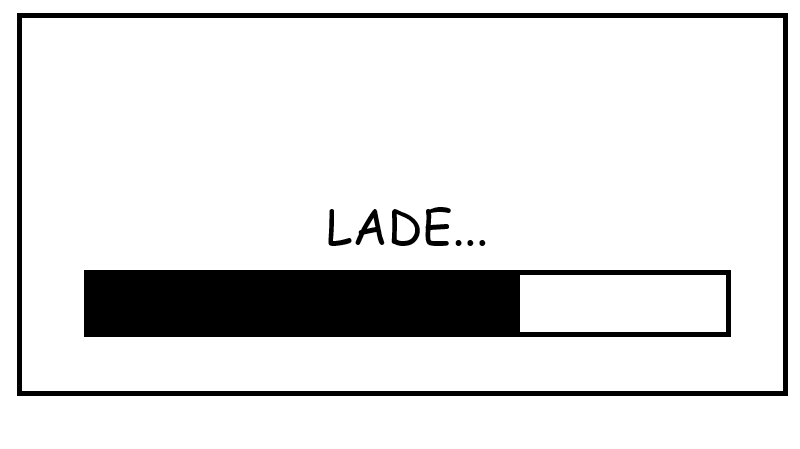
\includegraphics[width=\textwidth, height=7.5cm]{assets/LoadScreen}
	\end{minipage}
	
	\begin{minipage}{1\textwidth}
		\item \subsection*{Profilmenü:}
		Das Profilmenü öffnet sich unmittelbar nach erfolgreicher Beendigung des Ladevorgangs(Nähere informationen zum Ablauf und Ausnahmen folgen im Kapitel Szenarien).
		In diesem Menü kann der Spieler aus den bestehenden Spielerprofilen auswählen oder in das Menü zum anlegen eines neuen Spielers gelangen.\\
		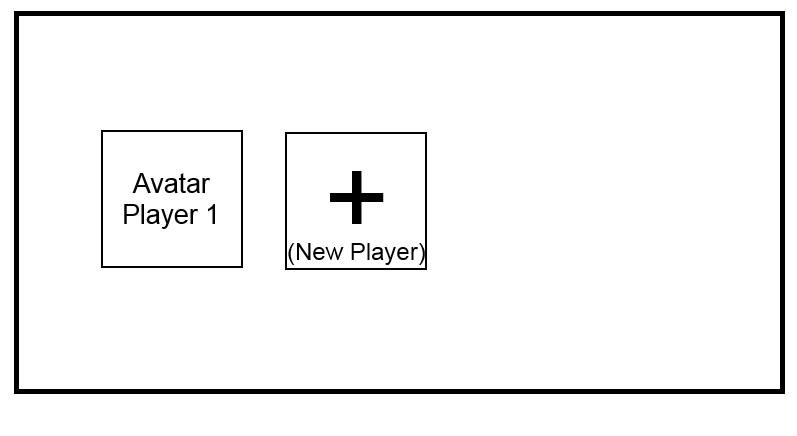
\includegraphics[width=\textwidth, height=7.5cm]{assets/PlayerScreen}
	\end{minipage}
	
	\begin{minipage}{1\textwidth}
		\item \subsection*{Profil anlegen:}
		In diesem Menü kann ein neues Spielerprofil vom Spieler angelegt werden. Der Spieler kann einen Namen für das Profil eingeben und aus einer gegebenen Menge an Avataren einen als Identifikationsmerkmal aussuchen.Sollte der Spieler hier abbrechen, so gelangt er zurück ins Profilmenü, ansonsten landet er entweder im Tutorial oder im Hauptmenü(Mehr dazu im Kapitel Szenarien)\\
		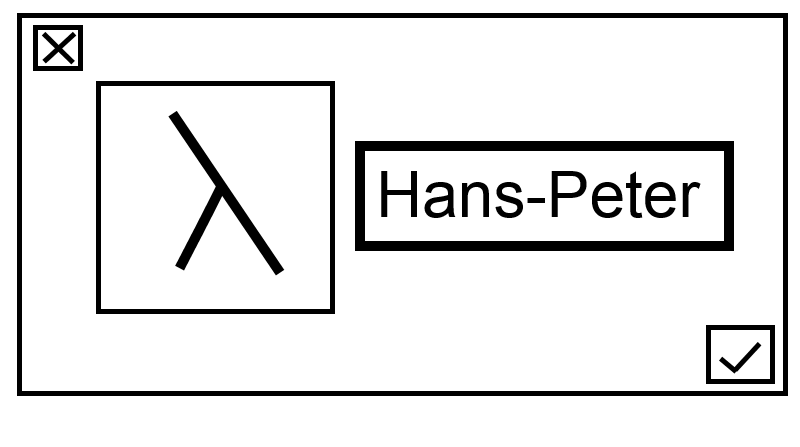
\includegraphics[width=\textwidth, height=7.5cm]{assets/CreateProfile}
	\end{minipage}
	
	\begin{minipage}{1\textwidth}
		\item \subsection*{Hauptmenü:} \label{appaufbau:Hauptmenü}
		Dies ist der Zentrale Knotenpunkt der App. von hier aus kann der Spieler zur Stageauswahl, den Einstellungen, seiner Statistik, zurück ins Profilmenü gelangen oder das Spiel komplett verlassen.\\
		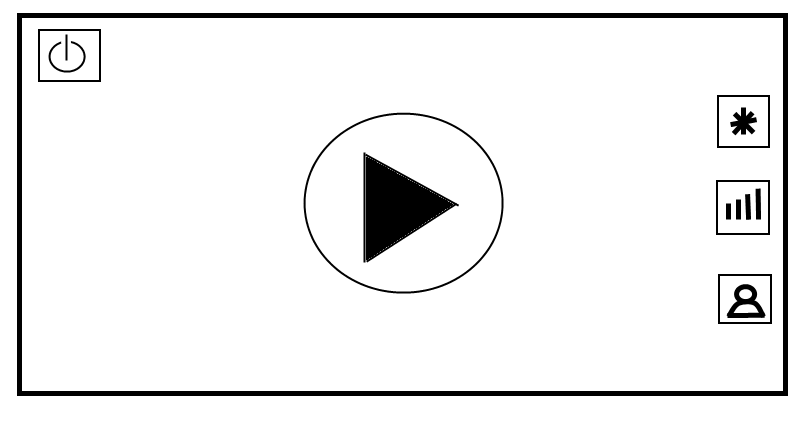
\includegraphics[width=\textwidth, height=7.5cm]{assets/Mainmenu}
	\end{minipage}
	
	\begin{minipage}{1\textwidth}
		\item \subsection*{Einstellungen:}
		Hier können verschiedene grundlegende Einstellungen vorgenommen werden. Außerdem gelangt man von hier ins Profilbearbeitungsmenü und zur Ansicht aller Achievments (Achievmentmenu).Der Zurück-Button führt ins Hauptmenü, beim verlassen werden sämtliche Änderungen gespeichert.\\
		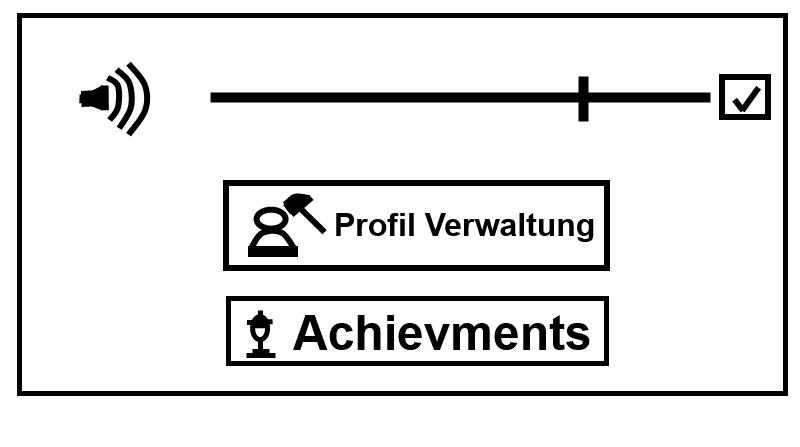
\includegraphics[width=\textwidth, height=7.5cm]{assets/Einstellungen}
	\end{minipage}

	\begin{minipage}{1\textwidth}
		\item \subsection*{Profilbearbeitungsmenü:}
		Dieses Menü ist absolut identisch mit dem Menü zum Anlegen eines neuen Spielerprofils. Der einzige Unterschied ist das jeder Weg aus diesem Menü zurück in die Einstellungen führt.\\
		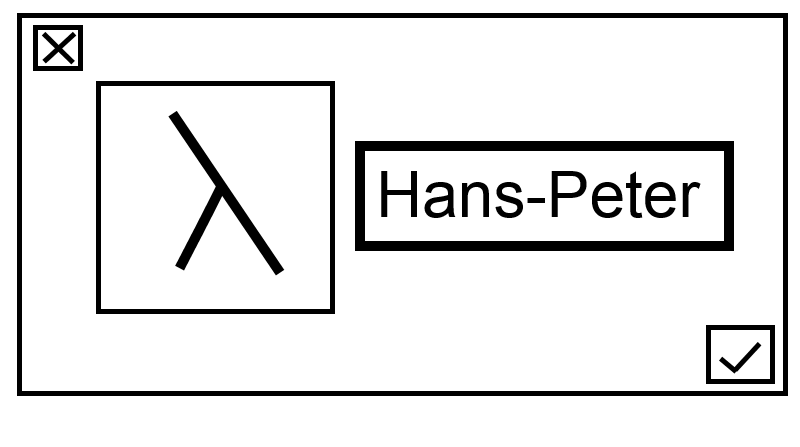
\includegraphics[width=\textwidth, height=7.5cm]{assets/CreateProfile}
	\end{minipage}

	\begin{minipage}{1\textwidth}
		\item \subsection*{Achievments:}
		Hier sind alle Achievments zu sehen, die die man schon erlangt hat sind durch ein Bild gekennzeichnet, ansonsten ist dort ein Platzhalter zu sehen. Ein Abbruch führt zurück in die Einstellungen.\\
		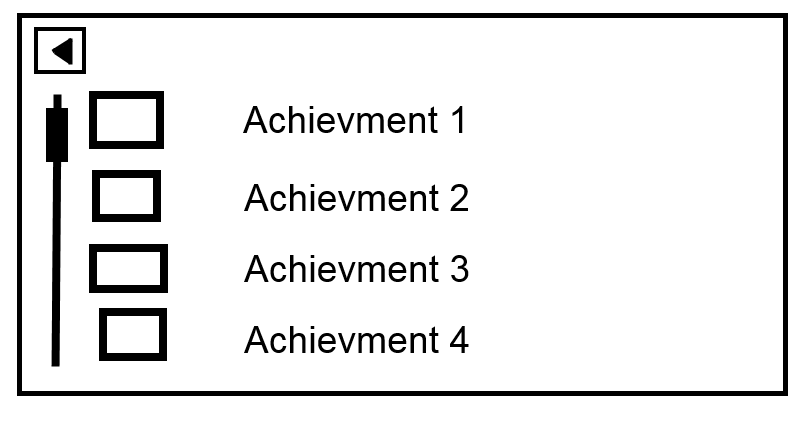
\includegraphics[width=\textwidth, height=7.5cm]{assets/Achievments}
	\end{minipage}
	
	\begin{minipage}{1\textwidth}
		\item \subsection*{Stagemenü:}
		Hier kann man sich eine Stage zum Spiele auswählen sie sind der Schwierigkeit nach geordnet und können im Spielverlauf freigeschaltet werden.\\
		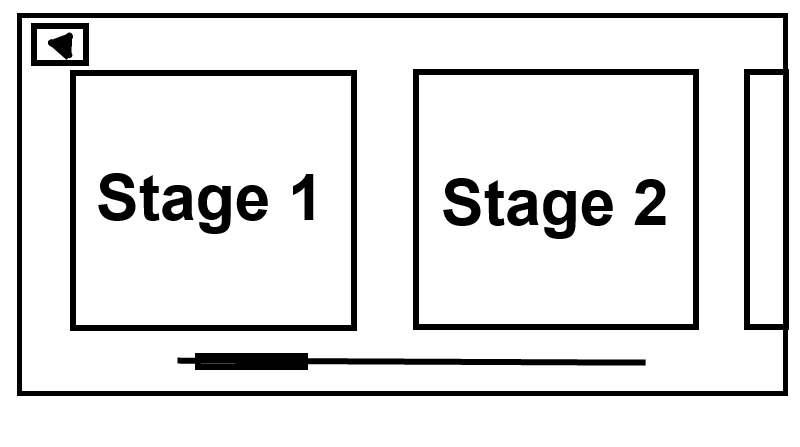
\includegraphics[width=\textwidth, height=7.5cm]{assets/Stagemenu}
	\end{minipage}
	
	\begin{minipage}{1\textwidth}
		\item \subsection*{Levelmenü:}
		hier kann ein Level der Stage in der man sich aktuell befindet gestartet werden.(auch diese müssen nach und nach freigeschaltet werden).\\
		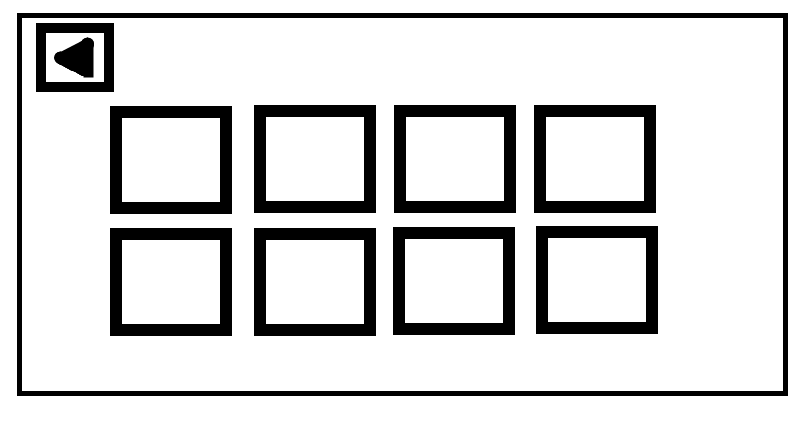
\includegraphics[width=\textwidth, height=7.5cm]{assets/Levelmenu}
	\end{minipage}
	
	\begin{minipage}{1\textwidth}
		\item \subsection*{Leveldesign:} \label{appaufbau:Leveldesign}
		Jedes Level hat den selben Grundaufbau. Am rechten Rand befindet sich eine Leiste aus der der Spieler per Drag and Drop die Spielelemente(siehe Spielaufbau) platzieren kann. Der Rest des Bildschirms nimmt das Spielfeld ein, auf dem zusätzlich am Rand Knöpfe zum Zoomen, dem aufrufen des Levelmenüs ,ansehen von Zielvorgabe und Hinweisen, sowie starten der Auswertung platziert sind.\\
		Das Levelmenü bietet die Auswahl zur Rückkehr ins Level(auswahl)menü, Hauptmenü, Neustarten des Levels und Rückkehr ins Level.\\
		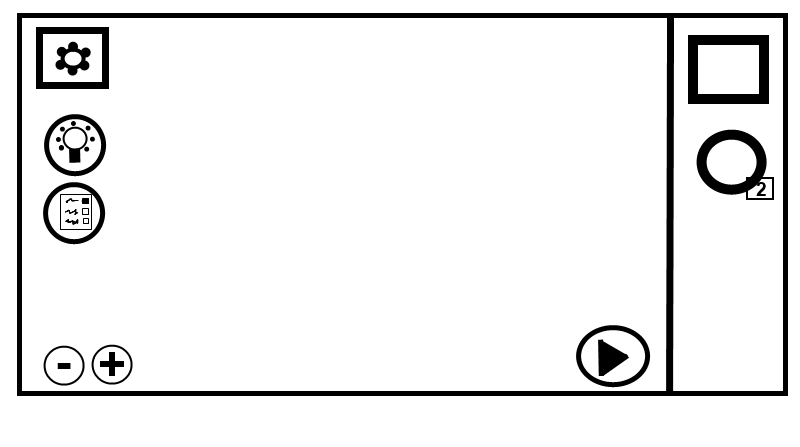
\includegraphics[width=\textwidth, height=7.5cm]{assets/LevelDesign}
	\end{minipage}
	
	\begin{minipage}{1\textwidth}
		\item \subsection*{Auswertungsmenü:}
		Hier erfährt der Spieler ob er das Level richtig gelöst hat oder nicht.
		Im Falle des Erfolgs kann der Spieler zurück zm Hauptmenü oder das nächste Level starten.
		Sollte er es nicht geschafft haben, kann er zurück zum Hauptmenü oder das Level Neustarten. Auch freigeschaltete Achievments werden hier angezeigt.\\
		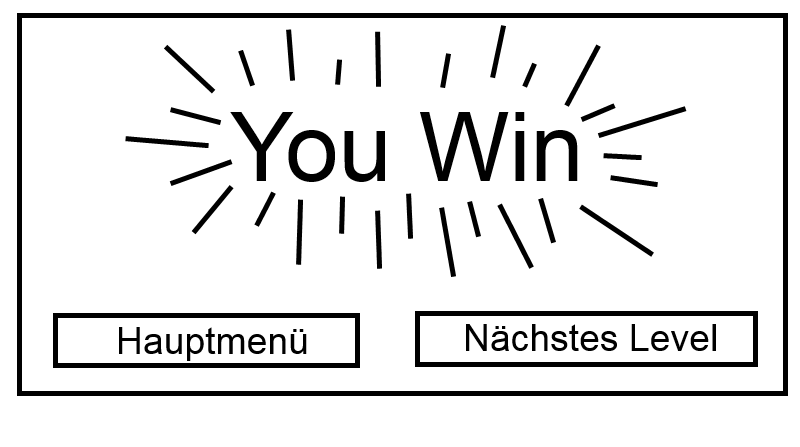
\includegraphics[width=\textwidth, height=7.5cm]{assets/Auswertungsmenu}
	\end{minipage}

\end{enumerate}

\clearpage














% ---------------
% Szenarien
% ---------------
\section{Szenarien}

\subsection{Erstes Ausführen des Spieles}
	\begin{enumerate}
		\item Starten der Applikation durch Anklicken der App-Verknüpfung
		\item Der Ladebildschirm(\ref{appaufbau:Ladebildschirm}) wird sichtbar und informiert über den Ladezustand des Spieles.
		\item Der Spieler wird direkt zum "Benutzer-Anlegen"  weitergeleitet
		\item Wurde ein Benutzer angelegt, öffnet sich die Einstellung
		\item Geht der Spieler von den Einstellungen weiter, beginnt der Tutorial-Modus
		\item Lamdbalino begrüßt den Spieler
		\item Es wird in die Handlung des Spieles eingeführt
		\item Nach dem Tutorial-Modus öffnet sich das Levelmenü und das erste Level ist freigeschaltet 
	\end{enumerate}
	
\subsection{Benutzer-Profil anlegen} \label{szenarien:ProfilAnlegen}
	\begin{enumerate}
		\item "Benutzer-Profil anlegen" wurde gewählt
		\item Der Spieler wählt einen Avatar
		\item Er gibt seinen Namen an
		\item Er kann wählen, ob er Rechtshänder oder Linkshänder ist
		\item Mit dem "Menü"-Knopf kommt der Benutzer ins Hauptmenü (\ref{appaufbau:Hauptmenü})
	\end{enumerate}	
	
\subsection{Tutorial-Modus}
	\begin{enumerate}
		\item Das Auswählen des Levels wird animiert
		\item Die Elemente des Spieles werden erklärt
		\item Ein Level wird Schrittweise simuliert
		\item Es öffnen sich kleine Felder um die nächste Handlung animiert zu erklären
		\item Schließt man die Felder, geht das Tutorial weiter
		\item Wie die Level, wird gezeigt wie die Maschinen funktionieren und wie sie angeordnet werden müssen
	\end{enumerate}
	
\subsection{Allgemeiner Spielstart}
	\begin{enumerate}
		\item Starten der Applikation durch Anklicken der App-Verknüpfung
		\item Der Ladebildschirm(\ref{appaufbau:Ladebildschirm}) wird sichtbar und informiert über den Ladezustand des Spieles
		\item Nach dem Laden kann man den Benutzer aus vorhandenen Profilen auswählen oder man legt ein neues Profil (\ref{szenarien:ProfilAnlegen}) an
		\item Das Hauptmenü (\ref{appaufbau:Hauptmenü}) wird geöffnet		
	\end{enumerate}
	
\subsection{Spielen} 
	\begin{enumerate}
		\item Im Hauptmenü wählt man die Stages
		\item In den Stages wählt man das Level (\ref{appaufbau:Leveldesign})
		\item Nach dem Öffnen des Levels, wird angezeigt, was die Maschine(n) produzieren müssen
		\item Möchte der Spieler erneut das gewünschte Produkt ansehen, kann er dies durch einen Knopf wählen
		\item Er spielt nach den Spielregeln (\ref{spielaufbau:Spielregeln})
		\item 
	\end{enumerate}
	
\subsection{Einstellungen}

\subsection{Benutzer-Profil bearbeiten}

\subsection{Informationen aufrufen}

\subsection{Statistiken}

\subsection{Achievements}

\subsection{Hauptmenü}

\subsection{Spiel verlassen}
	\begin{enumerate}
		\item Spiel beenden
			\begin{enumerate}
				\item 
			\end{enumerate}
		\item Spiel über das Betriebssystem verlassen
			\begin{enumerate}
				\item 
			\end{enumerate}
	\end{enumerate}


\end{document}